\chapter{La memoria cache dei principali Web Browser}

La memoria cache, propria di ogni browser, risiede all'interno di una directory all'interno del disco. 

Le modalità con le quali le informazioni presenti in cache vengono mantenute, la struttura della directory, i vari file che la compongono ed i collegamenti fra di essi variano fra i vari browser presi in esame. 

Il grafico sottostante mostra le percentuali di diffusione fra gli utenti dei maggiori browser, prendendo in esame un periodo di sei mesi.

\begin{figure}[htpb]
	\begin{center}
		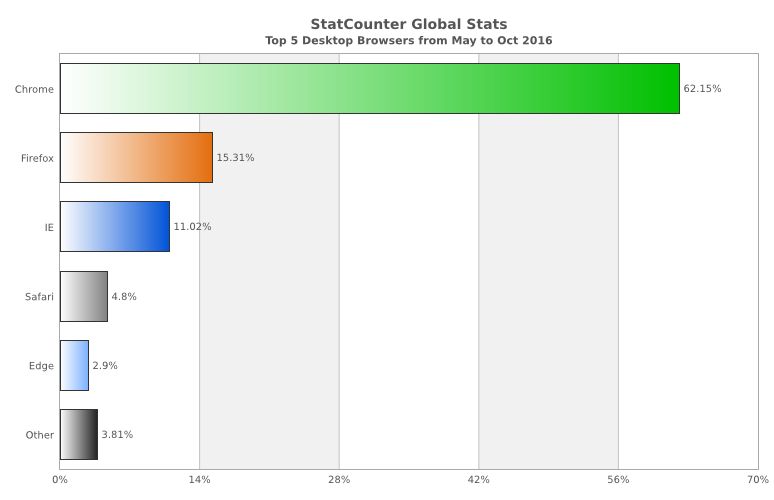
\includegraphics[scale=0.55]{StatCounter_browser_201605_201610_bar.png}
	\end{center}
\caption[Popolarità dei web browsers mag 2016 - ott 2016]{Popolarità dei web browser mag 2016 - ott 2016\footnotemark}
\end{figure}
\footnotetext{Fonte: \url{http://gs.statcounter.com/\#desktop-browser-ww-monthly-201605-201610-bar}} 

\section{Google Chrome}

Lanciato nel 2008 da parte di Google sulla base del progetto open source \textbf{Chromium}, il browser Google Chrome risulta esserne la versione compilata e distribuita da Google.
Al suo rilascio, nel settembre 2008, è stato reso pubblico anche il codice sorgente alla base di Chromium, con lo scopo di utilizzarlo come \textit{core} open source dell'applicazione, sottoponendolo nel frattempo alla revisione del codice da parte della comunità\footnote{Fonte: \url{http://www.google.com/intl/it/chrome/timemachine/}}. 
Rispetto a Chromium, il cui sviluppo ed i suoi rilasci sono gestiti dalla comunità di sviluppatori, Google Chrome viene distribuito ed aggiornato da Google stessa secondo una propria tabella di marcia.
Le differenze fra i due browser si notano principalmente nella natura \textit{open source} o \textit{closed source}, con Google Chrome che annovera anche estensioni e plugin closed source al contrario di Chromium.\footnote{Fonte:    \url{https://chromium.googlesource.com/chromium/src/+/master/docs/chromium_browser_vs_google_chrome.md}}

La struttura e gestione della memoria cache risulta essere uguale fra i due browser.

\subsection{Struttura della memoria cache}

I file componenti la cache sono mantenuti in una cartella sul disco la cui locazione di default dipende dal sistema operativo in uso. Per sistemi Windows si ha: 

\begin{itemize}
	\item{\texttt{C:\textbackslash Users\textbackslash\%Username\%\textbackslash AppData\textbackslash Local\textbackslash Google\textbackslash Chrome\textbackslash User Data\textbackslash Default\textbackslash Cache}}
\end{itemize}

Nella cartella della cache sono presenti almeno 5 files: un file \textbf{\textit{index}}, e 4 \textbf{\textit{data\_\# \footnote{Il \# indica un numero progressivo a partire da 0}}}. Altri file, detti \textbf{\textit{separate file}}, contengono informazioni la cui dimensione è maggiore di quella massima consentita per i file \textbf{\textit{data\_\#}}.

\begin{figure}[h]
	\centering
	\begin{minipage}[c]{0.6\textwidth}
		\dirtree{%
			.1 \textit{\textbf{GOOGLE CHROME CACHE FOLDER}}.
			.2 \textbf{Index File} \DTcomment{//Sempre presente}.
			.2 \textbf{Block Files} \DTcomment{//Sempre presenti}.
			.3 \textit{data\_0}.
			.3 \textit{data\_1}.
			.3 \textit{data\_2}.
			.3 \textit{data\_3}.
			.2 \textbf{Separate Files}  \DTcomment{//Opzionali}.
			.3 \textit{f\_\#\#\#\#\#\#}.
			.3 \vdots.
			.3 \vdots.
			.3 \textit{f\_\#\#\#\#\#\#}.
		} 
	\end{minipage}
	\caption{Struttura della cartella \textbf{\textit{cache}} di Chrome}
\end{figure}

\subsection{Struttura dei file}
Il file \textbf{\textit{index}} si presenta come una struttura formata da un \textit{index header} e da una \textit{tabella hash}. Il numero di elementi presenti è definito dal parametro \textit{table\_len} presente nell'header. 

Gli elementi contenuti nella tabella hash sono rappresentati secondo il formato \textbf{\textit{little endian}}. Ognuno di essi esprime il nome della risorsa (\textbf{\textit{key}}) e l'indirizzo in cache che la contiene. Convertendo in formato binario a 32 bit ed analizzando le varie sezioni si ottiene la locazione esatta (file e posizione al suo interno) di una risorsa che presenta lo stesso \textit{hash}.

\begin{savenotes}
	\begin{table}[H]
		\rowcolors{2}{lightgray}{white}
		\begin{center}
			\resizebox{0.65\textwidth}{!}{
			\begin{tabular}{c|c|c}
				\textbf{Offest} &\textbf{Size} &\textbf{Description}\\  \hline
				If file type is 0 (Separate file) \\
				0.0 &28 bits &File number \footnote{Valore di \# in f\_\#\#\#\#\#\#}\\
				Else \\
				0.0 &16 bits &Block number \\
				2.0 &8 bits &File number (or file selector) \footnote{Valore di \# in data\_\#}\\
				3.0 &2 bits &Block size \footnote{Numero di blocchi contigui: 0 rappresenta 1 blocco, 3 rappresenta 4 blocchi}  \\
				3.2 &2 bits &Reserved\\
				Common \\
				3.4 &3 bits &File type\\
				3.7 &1 bits &Initialized flag\\			
			\end{tabular}}
		\end{center}
		\caption{Struttura di un indirizzo cache di Chrome}
	\end{table}
\end{savenotes}

\begin{table}[H]
	\rowcolors{2}{lightgray}{white}
	\begin{center}
		\resizebox{0.85\textwidth}{!}{
			\begin{tabular}{c|c|c|c|c|c|c}
				&Init &File type &Reserved &Contiguous blocks &File number  &Block number \\ \hline
				Binary &1 &010 &00 &00 &0000 0001 &0000 0000 0000 0011 \\
				Integer &1 &2 &0 &0 &1 &3 
			\end{tabular}}
	\end{center}
	\caption{Esempio di un indirizzo cache di Chrome}
\end{table}

Interpretando il campo \textit{file type} nell'indirizzo si ottiene il file contenente la risorsa.
	
\begin{table}[H]
	\rowcolors{2}{lightgray}{white}
	\begin{center}
		\resizebox{0.6\textwidth}{!}{
		\begin{tabular}{c|c|c}
			\textbf{Binary} &\textbf{Integer} &\textbf{Interpretation}\\  \hline
			000 & 0 &Separate file\\
			001 & 1 &Ranking (36 byte block file)\\
			010 & 2 &256 byte block file\\
			011 & 3 &1 KByte block file\\
			100 & 4 &4 KByte block file\\
		\end{tabular}}
	\end{center}
	\caption{Tipi di file presenti nella cache di Chrome}
\end{table}


I \textbf{\textit{data\_\#}} file, indicati anche come \textbf{\textit{block file}}, sono costituiti da un header seguito da un numero variabile di blocchi aventi dimensione fissa. Il numero di blocchi presenti in un file di questo tipo è circa 64000. Se venisse richiesta la presenza di ulteriori blocchi della stessa dimensione, un nuovo file viene creato e collegato al precedente mediante il campo \textit{next\_file} presente nell'header. 
All'interno dei block file le informazioni vengono memorizzate utilizzando un massimo di 4 blocchi consecutivi. Se la dimensione dell'informazione da memorizzare dovesse superare quella di 4 blocchi consecutivi, questa viene memorizzata in una di dimensioni maggiori.
\newline

I \textbf{\textit{separate file}} del tipo \textit{f\_\#\#\#\#\#\#} invece memorizzano le informazioni di dimensioni maggiori di 16 KB. 
Il loro nome è nella forma f\_ seguito da un numero esadecimale progressivo di 6 cifre. 
Questo tipo di file non presenta header ma contiene solamente dati.
\newline

Sia le risorse di dimensioni fino a 16 KB nei \textit{data\_\# file}, sia quelle di dimensioni maggiori che risiedono nei \textit{f\_\#\#\#\#\#\#}, sono memorizzate in formato \textbf{\textit{gzip}}. 
\clearpage

\begin{figure}[htpb]
	\begin{center}
		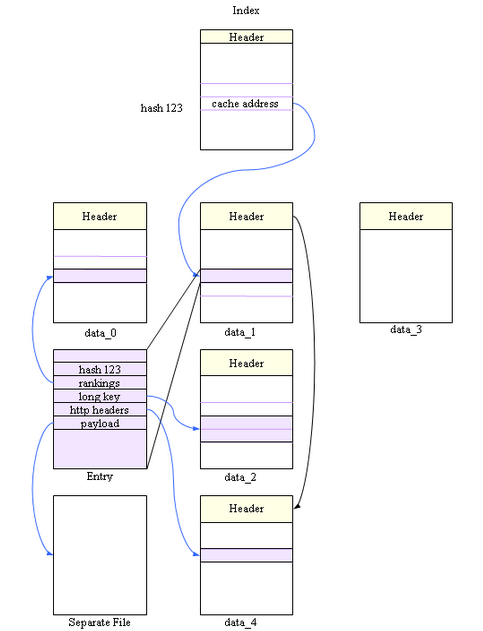
\includegraphics[scale=0.8]{Chrome_cache_overview.png}
	\end{center}
	\caption[Diagramma della cache di Chrome]{Diagramma della cache di Chrome}
\end{figure}
\footnotetext{Fonte: \url{https://www.chromium.org/developers/design-documents/network-stack/disk-cache}}




 
